\documentclass[sigconf,review,anonymous]{acmart}

%% FSE 2027 Research track --- W5 SameEval rewrite (2026-09-16). Not camera-ready.
%% Double-blind: keep anonymous/review until camera-ready.
\acmConference[FSE '27]{ACM International Conference on the Foundations of Software Engineering}{July 12--16, 2027}{Shenzhen, China}
\acmBooktitle{Proceedings of the ACM International Conference on the Foundations of Software Engineering (FSE '27), July 12--16, 2027, Shenzhen, China}
\copyrightyear{2027}
\acmYear{2027}
\setcopyright{none}

\usepackage{booktabs}
\usepackage{graphicx}
\usepackage{amsmath}

\newcommand{\skyt}{\textsc{Skyt}}
\newcommand{\sameeval}{SameEval}
\newcommand{\sameat}{\mbox{\texttt{same@2}}}
\newcommand{\sameatc}{\mbox{\texttt{same@2|cert}}}
\newcommand{\etal}{et~al.}
\newcommand{\ie}{i.e.,}
\newcommand{\eg}{e.g.,}

%% ---------- DRAFTING NOTES (LaTeX comments only; do not print) ----------
%% C1 SameEval overlay: N regenerations + canonical-form fingerprint + same@2.
%% C2 Measure ≠ policy: first-valid vs Certified Consensus; SKYT is the tool.
%% C3 Empirical: contracted tasks + HumanEval+ Table 1 = 164 N=20 overlay.
%% C4 SKYT scored on contracted tasks only (Results A). No HumanEval+ SKYT table.
%% Protocol N=20 / s=10. Table 1 is that protocol on all 164 tasks.
%% Never merge SBES (12/3600), MSR (15/4500), HumanEval+ 164/13120.
%% Do not headline split-half medoid 74.3%. 66pp is anchor-relative only.
%% HumanEval+ is the 164-task N=20 overlay only. No SKYT on HumanEval+.
%% Code DNA / IVR is out of scope. Do not score SKYT by pass@k or match-to-human.
%% -----------------------------------------------------------------------

\begin{document}

\title{\sameeval{}: Measuring Whether Regenerated Code Is the Same Program}

%% Blind review: authors commented until camera-ready.
%% \author{Heitor Roriz}
%% \affiliation{%
%%   \institution{Massimus}
%%   \city{S\~{a}o Paulo}
%%   \country{Brazil}
%% }
%% \email{heitor@massimus.com}
%%
%% \author{Nasser Jazdi-Motlagh}
%% \affiliation{%
%%   \institution{University of Stuttgart}
%%   \city{Stuttgart}
%%   \country{Germany}
%% }
%% \email{nasser.jazdi@ias.uni-stuttgart.de}
%%
%% \author{Vicente Lucena}
%% \affiliation{%
%%   \institution{Federal University of Amazonas}
%%   \city{Manaus}
%%   \country{Brazil}
%% }
%% \email{vicente@ufam.edu.br}

\renewcommand{\shortauthors}{Anonymous Author(s)}
\renewcommand{\shorttitle}{\sameeval{}: Is Regenerated Code the Same Program?}

\begin{abstract}
Code-generation benchmarks ask whether a generated program passes tests, but
real development workflows often regenerate code from the same prompt.
A passing sample therefore does not tell us whether the next successful sample
will have the same structure.

We introduce \sameeval{}, a benchmark overlay for measuring structural
repeatability in LLM-generated code. For each task, model, and temperature
configuration, \sameeval{} draws multiple independent generations, evaluates
them using the existing behavioral oracle, maps structurally valid outputs to
canonical-form fingerprints, and reports \sameat{}: the probability that two
independent generations both certify and have the same canonical form.
We additionally report \sameatc{}, which measures structural agreement among
successful generations.

Across two contracted-task corpora comprising 8{,}100 generations, behavioral
pass rates exceed 98\%, \sameat{} is 61.0\% and 67.5\%, and \sameatc{} is
66.5\% and 68.9\%, respectively.
On 13{,}120 generations from 164 HumanEval+ tasks, plus-pass is 83.3\%,
\sameat{} is 65.9\%, and \sameatc{} is 76.6\%.
\sameat{} is a pairwise U-statistic with failures in the denominator; it is
not a pass rate and is not comparable to pass$^2$.
Among certified pairs, a substantial share still disagree on form.

\sameeval{} further separates that measurement from the policy used to select
a reference form. Using \skyt{} as a post-generation canonicalizer on the
contracted-task corpora, certified-consensus repair raises \sameat{} to
77.2\% and 85.2\%.
Those figures are in-sample batch canonicalization of the same draws that
voted for the consensus form, not evidence that the generator became more
repeatable.
This paper does not report \skyt{} on HumanEval+.

\sameeval{} adds a complementary dimension to code-generation evaluation:
whether repeated successful generations converge to the same program form.
\end{abstract}

\keywords{LLM code generation, structural repeatability, \sameeval{}, \sameat{}, HumanEval+, software measurement}

\maketitle

\section{Introduction}
\label{sec:intro}

Correctness benchmarks for LLM code generation---HumanEval~\cite{chen2021evaluating},
MBPP~\cite{austin2021program}, SWE-bench~\cite{jimenez2024swebench}---ask whether
\emph{a} generated artifact passes tests.
Production pipelines regenerate: CI retries a generator, an agent re-samples
after a failed test, and two developers issue the same prompt.
Tests cannot tell two passing regenerations apart, yet the artifacts can
differ in structure~\cite{ouyang2023llm}.

This paper's primary contribution is \textbf{\sameeval{}}, a benchmark overlay
that measures that scatter.
It ships no new prompts and no new tests.
It adds a form report on top of an existing task set.
The report's headline is \sameat{}: the probability that two independent draws
both certify and are the same program.
A second column, \sameatc{}, asks the same identity question among passers
only; configs with fewer than two passers are dropped from that column and the
drop is reported.

\sameeval{} does not pick a canon and does not aim at a shipped human solution.
``Same form'' means identical canonical-form fingerprints
(Section~\ref{sec:sameness}).
Which verified form, if any, later generations should be repaired toward is a
\emph{policy}, not a measurement.
We compare first-compliant repair to Certified Consensus repair on contracted
tasks, scoring a post-generation tool, \skyt{}~\cite{roriz2026skytmsr},
before and after, never mixed into the raw overlay.

We apply \sameeval{} to author-written contracted tasks (Results~A) and to all
164 HumanEval+~\cite{liu2023evalplus} tasks at protocol $N{=}20$
(Results~B, Table~\ref{tab:he-table1}).
SBES, MSR, and HumanEval+ numbers are never pooled.

\paragraph{Not in this paper.}
Generation-by-construction (``Code DNA'') is a separate vision paper.
We do not claim MISRA~C~\cite{misra2012} or NASA Power-of-10~\cite{holzmann2006power}
compliance for any contract.
We do not score \skyt{} by pass@$k$ or by match to the HumanEval canonical
solution.
We do not report \skyt{} on HumanEval+.

\paragraph{Outline.}
Section~\ref{sec:motivation} records a measured review cost.
Section~\ref{sec:related} places \sameeval{} next to pass@$k$, clones, and
repair.
Section~\ref{sec:protocol} defines the overlay and separates measurement from
canon policy.
Section~\ref{sec:setup} pins the two corpora.
Section~\ref{sec:results-a} reports contracted-task scores under both repair
policies.
Section~\ref{sec:results-b} reports HumanEval+ \sameeval{} scores.
Section~\ref{sec:threats} states construct caveats.
Section~\ref{sec:artifact} lists hashes, seeds, and recompute commands.

\section{Motivation}
\label{sec:motivation}

Regeneration is how LLM-assisted development actually works.
Correctness benchmarks record whether \emph{a} sample
passes~\cite{chen2021evaluating,liu2023evalplus}.
They do not record whether the next passing sample is the same program.

\paragraph{Review cost, measured.}
Conditioned on generations that already pass, mean line-level churn between a
random pair is 13.1\% (MSR) and 13.8\% (SBES): about 2.7 changed lines on
$\approx$12-line functions.
Churn tracks temperature: 3.2\% at $T{=}0.0$ to 23.1\% at $T{=}1.0$.
The test suite treats those pairs as interchangeable; a reviewer does not.

\paragraph{Keeping the first passer is a policy.}
A natural operational response is to freeze the first program that certifies.
On contracted tasks that first certified generation matches the certified
consensus form in only 40.5\% of MSR configs that have a consensus
(40.6\% SBES).
Commercial APIs are not bit-deterministic at
$T{=}0$~\cite{ouyang2023llm}.
Freezing one output works until anyone re-runs the prompt.

That is the measurement problem \sameeval{} is for.

\section{Related Work}
\label{sec:related}

\paragraph{Functional correctness.}
HumanEval~\cite{chen2021evaluating}, MBPP~\cite{austin2021program}, and
SWE-bench~\cite{jimenez2024swebench} score pass@$k$ against tests.
HumanEval+~\cite{liu2023evalplus} keeps the same 164 prompts and replaces the
hidden tests with a larger extra suite.
These protocols do not report how often independent draws share structure.
AlphaCode~\cite{li2022alphacode} clusters programs by input--output behavior to
filter duplicate submissions; that is a selection policy, not a population
report.

\paragraph{LLM variability.}
Ouyang \etal{}~\cite{ouyang2023llm} document non-determinism in code
generation, including that $T{=}0$ is not bit-deterministic on commercial
APIs; temperature changes output diversity~\cite{zhu2024hot}.
ReCode~\cite{wang2023recode} perturbs \emph{prompts} and asks whether pass
rate holds.
\sameeval{} leaves the prompt fixed and asks whether two answers are the same
program.
Studies of developer interaction~\cite{vaithilingam2022expectation,barke2023grounded}
treat a generation as a single artifact.

\paragraph{Clones and diffs.}
Fingerprint identity is closer to clone measurement than to
pass@$k$~\cite{roy2009clone}.
AST differencing~\cite{falleri2014gumtree} produces an edit script between two
trees; Zhang--Shasha tree-edit distance~\cite{zhang1989simple} is a related
numeric judge.
\sameeval{} asks how often independent regenerations land on the same
canonical form.
It is not a clone detector, not observational equivalence, and not algorithm
identity.
Clone and TED judges are not written into \sameat{}.

\paragraph{Repair versus overlay.}
Program repair with language models patches failing
code~\cite{xia2023apr}.
\skyt{} is a post-generation canonicalizer toward a stored verified
form~\cite{roriz2026skytmsr}, not a bug fixer and not a generator.
\sameeval{} is the overlay: same tasks, extra form reports.
\skyt{} is one system scored on that overlay.

\section{\sameeval{}}
\label{sec:protocol}

\subsection{Inputs and regenerations}
A \emph{task} supplies a prompt, a behavioral oracle (unit tests), and optional
static constraints (a \emph{contract}).
An experimental \emph{config} is one task $\times$ one model $\times$ one
temperature.
For each config we draw $N$ independent generations.
The \sameeval{} protocol uses $N{=}20$ (cross-validation train size $s{=}10$).
HumanEval+ Table~\ref{tab:he-table1} is that protocol on all 164 tasks.

\subsection{Certification}
\label{sec:certification}
\emph{Certified} is a predicate on a generation, and it is not the same on both
datasets.
On contracted tasks, certified means the behavioral oracle passes \emph{and}
the contract checker passes.
On HumanEval+, certified means the HumanEval+ extra tests (plus) pass.
Original HumanEval (base) tests are stored and are never mixed into
certification.
Unparseable code is structurally invalid; it cannot certify, but it stays in
the \sameat{} denominator.

\subsection{Structural sameness}
\label{sec:sameness}
Two generations are the \emph{same form} iff both parse and their canonical-form
fingerprints match.
The canonical form is: parse to an AST; strip leading docstrings from every
module, function, and class body; $\alpha$-rename bound parameters and locals
when the task's naming policy is flexible (free names stay); unparse so the
tree and the source agree; hash \texttt{ast.dump} of that tree.

\skyt{} still extracts a vector of 14 properties for the \emph{tool}.
Those extras are diagnostics of \emph{how} two forms differ.
They are not conjuncts of \sameeval{} identity.
A previously used behavioral-signature extractor is disabled because it
executed generated code.

Distance 0 on the fingerprint is not semantic equivalence
(Section~\ref{sec:threats}).

\subsection{Population measures}
\label{sec:measures}
Let a config have $N$ generations and write $C(N,2)$ for the unordered pairs.

\begin{enumerate}
  \item \textbf{\sameat{}} (primary).
        The fraction of pairs in which both generations are certified and have
        the same form.
        \[
          \texttt{same@2}
          \;=\;
          \frac{\#\{\{i,j\}\,:\,\text{both certified and same form}\}}{C(N,2)}.
        \]
        This is a U-statistic of order 2.
        Failures remain in the denominator.
        It is defined on every config.
  \item \textbf{\sameatc{}} (secondary).
        The same identity check restricted to pairs of certified generations.
        Undefined when fewer than two generations certify; those configs are
        omitted from the mean of this column and the omission is reported.
  \item \textbf{Certified modal mass.}
        Size of the largest certified same-form class, divided by $N$
        (failures count).
\end{enumerate}

Always report \sameat{}, \sameatc{} (with the drop count), and pass rate
together, with $N$ and the task count in the same sentence as the headline.
Reporting \sameatc{} alone is forbidden: it rises when the pass rate falls.

Pairs within a config share generations and are not independent Bernoulli
trials.
Inference aggregates \emph{one score per task} (or contract) and uses a
cluster bootstrap (10{,}000 resamples, seed 20260723).
We do not treat $C(N,2)$ pairs as binomial trials and do not put a Wilson
interval on in-sample modal share.

\subsection{Canon policy (not part of \sameeval{})}
\label{sec:canon-policy}
\sameeval{} asks how scattered the outputs are.
A \emph{canon} is a chosen reference form used as a repair target or as a
held-out predictor.
That choice is a policy.
\skyt{} implements a policy; it is not the overlay.

\textbf{Certified Consensus.}
Among certified, structurally valid generations, form same-form equivalence
classes (transitivity checked).
Take the largest class (mode).
If several classes share that size, take their members as candidates.
Among candidates, pick the medoid relative to \emph{all other certified}
samples (smallest mean distance), then the lexicographically smallest source
string, then index.
The result is an observed generation.
If nothing certifies, there is no canon; repair is skipped.

\textbf{First-compliant (first-valid).}
Repair toward the first generation in the config that certifies.
This is the historical contracted-task baseline.
It is not the live repair target.

\textbf{Policy evaluation.}
Repeated balanced cross-validation: pick a consensus form on a train split of
size $s$, score \sameat{} on the complement.
On contracted tasks, $s{=}10$ ($N{=}20$), $B{=}2000$ splits, same seed.
Table~\ref{tab:he-table1} reports overlay scores at $N{=}20$ and has no CV column.
Leave-one-out and a single split-half are sensitivity only; we do not headline
the contracted-task split-half medoid (74.3\%).

The shipped HumanEval \texttt{canonical\_solution} is an external baseline, not
a \sameeval{} canon.

\section{Experimental Setup}
\label{sec:setup}

\subsection{Contracted tasks}
\label{sec:setup-contracts}
Two scopes, never pooled into one headline.
\textbf{SBES:} 12 contracts, 3{,}600 generations.
\textbf{MSR:} 15 tasks (12 base + 3 \texttt{\_strict} variants), 4{,}500
generations.
Models: GPT-4o-mini, GPT-4o, Claude Sonnet 4.5.
Temperatures: $\{0.0, 0.3, 0.5, 0.7, 1.0\}$.
$N{=}20$ per config.

Gate~0 analysis uses 220 complete configs (MSR grid 225 minus the entire
\texttt{is\_prime\_strict}$\times$Claude cell, 5 configs).
The three \texttt{\_strict} variants were not validated against a real MISRA~C
or NASA Power-of-10 rule set; those names are inspiration only.

Historical artifacts \texttt{outputs/*.json} and \texttt{outputs/gate0/} are
first-valid repair.
Certified Consensus repair was replayed without new LLM calls into a parallel
tree (\texttt{outputs/consensus\_repair/}, Gate~0 on that tree in
\texttt{outputs/gate0\_consensus/}).
If nothing certifies (\texttt{binary\_search\_strict}, 15 configs), raw
generations are copied through; no form is invented.

On this corpus, fingerprint identity and the older 14-property conjunction
agree on every same/different verdict, so contracted-task \sameat{} does not
depend on that choice.

\subsection{HumanEval+}
\label{sec:humaneval}
Prompts are the 164 HumanEval tasks.
The oracle is HumanEval+ extra tests~\cite{liu2023evalplus}, not the original
hidden file.
Dataset pin: \texttt{evalplus==0.3.1}, HumanEvalPlus \texttt{v0.1.10},
\texttt{dataset\_md5 = 916d9bfe7b490c2447245ec91595fa4f}.
This paper's Table~\ref{tab:he-table1} reports all 164 tasks at protocol $N{=}20$
(GPT-4o-mini and Claude Sonnet 4.5,
\texttt{claude-sonnet-4-5-20250929};
$T\in\{0.0,0.7\}$; 13{,}120 generations / 656 configs).
Completions are stitched onto the prompt and scored in network-disabled Docker
(\texttt{python:3.13-slim@sha256:7e3a6aca9d74f93cca21a91d86a8dad8c34749afd5b4a98ee481c9c47b9f5ed4}).
Untrusted code is not executed on the host.
There is no style or MISRA-style contract on this run: certified means plus
tests pass.
The human \texttt{canonical\_solution} is stored as an external baseline, not a
Table~\ref{tab:he-table1} column.

The overlay is scored with canonical-form fingerprints
(Section~\ref{sec:sameness}; \texttt{relation\_version}=2).

\subsection{Tool under test}
\label{sec:skyt}
\skyt{} is a post-generation canonicalizer, not a generating agent.
On contracted tasks, repair uses the labeled policy (first-valid or certified
consensus) and a property-based transformer, then re-runs the oracle and rolls
back if tests fail.
This paper does not apply \skyt{} to HumanEval+.

\section{Results A: Contracted Tasks}
\label{sec:results-a}

Figure~\ref{fig:overview} summarizes \sameat{} on contracted tasks (panel~a)
and the HumanEval+ 164-task overlay (panel~b).
The two corpora are never pooled.
Error bars are 95\% cluster bootstrap by contract or by task.

\begin{figure*}[t]
  \centering
  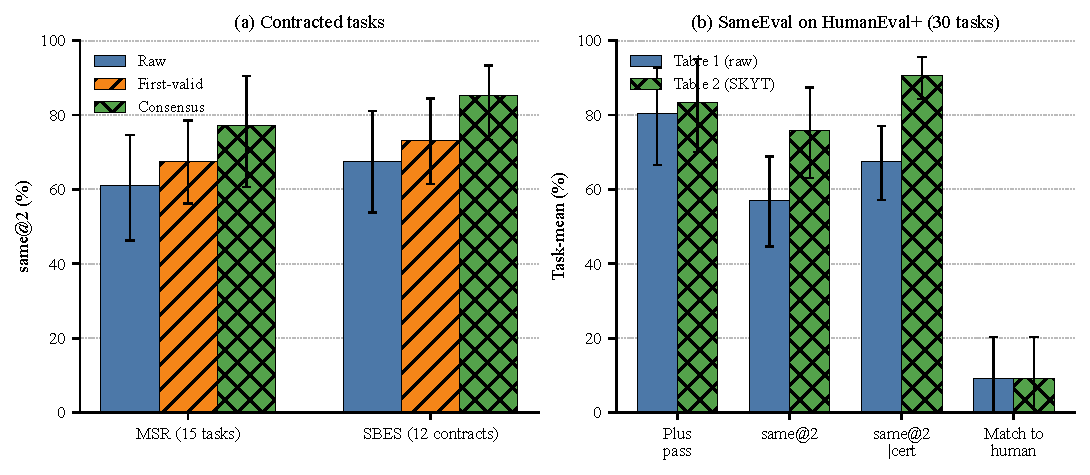
\includegraphics[width=\textwidth]{fig1.pdf}
  \caption{\sameeval{} scores.
    (a)~Contracted tasks: \sameat{} on raw generations, after first-valid
    repair, and after Certified Consensus repair.
    MSR (15 tasks, 4{,}500 generations) and SBES (12 contracts, 3{,}600
    generations) are separate groups.
    (b)~HumanEval+ 164-task overlay (13{,}120 generations, $N{=}20$):
    Table~\ref{tab:he-table1} is \sameeval{} only; \skyt{} is not applied to these programs.
    Whiskers are 95\% cluster bootstrap.}
  \label{fig:overview}
\end{figure*}

Table~\ref{tab:gate0-pre} reports \sameeval{} measures on the \emph{raw}
generations (repair policy does not change pre-repair scores).
Behavioral pass is 98.4\% (MSR) and 98.1\% (SBES).
\sameat{} is 61.0\% (MSR; 95\% cluster CI 46.3--74.6) and 67.5\% (SBES;
53.8--81.0).
\sameatc{} is 66.5\% (MSR; 205/220 configs) and 68.9\% (SBES; 180/180).
Certified modal mass is 69.6\% (MSR; 55.7--81.7) and 76.4\% (SBES; 65.5--87.0).
Held-out CV at $s{=}10$ is 67.5\% (MSR; 53.1--80.2) and 74.3\% (SBES; 62.2--85.9).
The form gap among certified pairs is 33.5\,pp (MSR) and 31.1\,pp (SBES)
below 100\% \sameatc{}.
Do not read 98\% pass versus 61\% \sameat{} as a 37\,pp form gap:
\sameat{} still includes failing draws.
An older $\approx$66\,pp figure compared behavioral pass to match against the
first certified generation; that gap is \textbf{anchor-relative} and is not a
headline.

\begin{table}[t]
  \caption{Pre-repair \sameeval{} measures on contracted tasks (contract-mean).
    Pairwise is \sameat{}.
    \sameatc{} drops configs with fewer than two certified generations
    (MSR 15/220; SBES 0/180).
    CV is repeated balanced held-out \sameat{} at $s{=}10$.
    Scopes are never merged.
    Cluster-bootstrap 95\% CIs for \sameat{}: MSR 46.3--74.6, SBES 53.8--81.0.
    The MSR split-half medoid (also $\approx$74.3\%) is not a headline and is
    not the SBES CV cell.}
  \label{tab:gate0-pre}
  \begin{tabular}{lccccc}
    \toprule
    Scope & Pass & \sameatc{} & \sameat{} & Modal & CV \\
    \midrule
    MSR (15 tasks)  & 98.4\% & 66.5\% & 61.0\% & 69.6\% & 67.5\% \\
    SBES (12 contracts) & 98.1\% & 68.9\% & 67.5\% & 76.4\% & 74.3\% \\
    \bottomrule
  \end{tabular}
\end{table}

\sameat{} keeps all 220 MSR configs.
The 15 MSR configs omitted from \sameatc{} are
\texttt{binary\_search\_strict} (0 certified generations; literal-pattern
constraints that generations did not satisfy).

Table~\ref{tab:gate0-post} reports the same measures after repair, with the two
policies labeled.
First-valid raises MSR \sameat{} 61.0\%$\rightarrow$67.4\% (CI 56.2--78.5) and
SBES 67.5\%$\rightarrow$73.2\% (61.4--84.4), with 69 MSR regressions / 0
rescues (post pass 96.8\%) and 14 SBES regressions / 0 rescues (post pass
97.7\%).
Fifty-five of the MSR regressions are \texttt{is\_prime\_strict}/GPT-4o.
Certified Consensus raises MSR \sameat{} to 77.2\% (60.7--90.4) and SBES to
85.2\% (73.2--93.3); \sameatc{} becomes 83.2\% and 85.8\%.
There are 0 regressions and 56 rescues in each scope (post pass 99.7\% MSR,
99.6\% SBES).
We report both policies and do not mix them into one number.
Those post-repair scores rewrite the same $N{=}20$ draws that voted for the
consensus form.

\begin{table}[t]
  \caption{Post-repair \sameeval{} measures on contracted tasks (contract-mean).
    Pairwise is \sameat{}.
    First-valid artifacts: \texttt{outputs/gate0/}.
    Consensus artifacts: \texttt{outputs/consensus\_repair/} and
    \texttt{outputs/gate0\_consensus/}.
    In-sample: the consensus form is picked from the same $N$ that is rewritten.
    Cluster-bootstrap 95\% CIs for \sameat{}: MSR first-valid 56.2--78.5,
    MSR consensus 60.7--90.4, SBES first-valid 61.4--84.4, SBES consensus
    73.2--93.3.}
  \label{tab:gate0-post}
  \begin{tabular}{llccccc}
    \toprule
    Scope & Policy & Pass & \sameatc{} & \sameat{} & Modal & CV \\
    \midrule
    MSR  & first-valid & 96.8\% & 75.1\% & 67.4\% & 75.4\% & 74.1\% \\
    MSR  & consensus   & 99.7\% & 83.2\% & 77.2\% & 82.2\% & 81.4\% \\
    SBES & first-valid & 97.7\% & 74.9\% & 73.2\% & 81.2\% & 79.9\% \\
    SBES & consensus   & 99.6\% & 85.8\% & 85.2\% & 90.1\% & 89.4\% \\
    \bottomrule
  \end{tabular}
\end{table}

First-valid matches Certified Consensus in 40.5\% of MSR configs that have a
consensus (40.6\% SBES).
The two policies are not the same center.

\section{Results B: \sameeval{} on HumanEval+}
\label{sec:results-b}

Table~\ref{tab:he-table1} is \sameeval{} on all 164 HumanEval+ tasks at
protocol $N{=}20$ (13{,}120 generations).
Those numbers are not pooled with SBES or MSR.
Aggregation is a task-mean with cluster bootstrap by \texttt{task\_id}
(10{,}000, seed 20260723).
Figure~\ref{fig:overview}(b) shows the overall.

Table~\ref{tab:he-table1} is overlay only (no \skyt{}).
Overall plus-pass is 83.3\% (95\% CI 78.3--88.0).
\sameat{} is 65.9\% (61.0--70.6).
\sameatc{} is 76.6\% (73.0--80.0) and is computed on 562/656 configs
(94 configs had fewer than two plus-passers and are omitted from that column
only).
$T{=}0.0$ is not 100\% \sameatc{}.
Plus-pass 83.3\% versus \sameat{} 65.9\% is not a 17\,pp form gap.
Independent Bernoulli certification at that pass rate would give
$\mathrm{pass}^2\approx 69\%$ even if every certified pair matched;
across-task heterogeneity makes the share of certified pairs larger than
$\mathrm{pass}^2$ (implied joint certification $\sameat{}/\sameatc{}\approx 86\%$).
The form disagreement among passers is $100\%-76.6\%=23.4$\,pp on \sameatc{}.

The overlay uses canonical-form fingerprints (\texttt{relation\_version}=2).
It does not report certified modal mass, held-out CV, or match to the shipped
human solution.

The cell that drives the structural story is GPT-4o-mini at $T{=}0.7$:
plus-pass 79.7\%, \sameatc{} 60.0\%, \sameat{} 48.9\%.
Tests pass; forms still differ.

\begin{table*}[t]
  \caption{\sameeval{} on HumanEval+, 164 tasks.
    Overlay only; no \skyt{}.
    $N{=}20$.
    CIs are 95\% cluster bootstrap by task.
    \sameatc{} drops configs with fewer than two plus-passers
    (94/656 omitted).}
  \label{tab:he-table1}
  \begin{tabular}{llccc}
    \toprule
    Model & $T$ & Plus pass & \sameatc{} & \sameat{} \\
    \midrule
    GPT-4o-mini & 0.0 & 79.3\% & 93.7\% & 74.3\% \\
    GPT-4o-mini & 0.7 & 79.7\% & 60.0\% & 48.9\% \\
    Claude Sonnet 4.5 & 0.0 & 87.4\% & 88.4\% & 77.3\% \\
    Claude Sonnet 4.5 & 0.7 & 86.8\% & 72.2\% & 63.2\% \\
    both & both & 83.3\% & 76.6\% & 65.9\% \\
    \bottomrule
  \end{tabular}
\end{table*}

\section{Discussion}
\label{sec:discussion}

Measurement and policy answer different questions.
Figure~\ref{fig:overview} and Tables~\ref{tab:gate0-pre}--\ref{tab:he-table1}
keep those questions apart.
Table~\ref{tab:gate0-pre} and Table~\ref{tab:he-table1} describe scatter of
samples.
Table~\ref{tab:gate0-post} describes contracted-task samples after a chosen
repair target; those scores are in-sample.
Certified Consensus is a center among verified forms, not a quality-best
program and not the HumanEval human file.

First-valid on contracted tasks improves structure less than consensus and
introduces regressions.
Consensus repair on those tasks improves structure with rescues rather than
regressions in the Gate~0 replay.
Those two sentences are why both policies are in the paper.

\section{Threats to Validity}
\label{sec:threats}

\paragraph{Two pairwise columns.}
\sameat{} keeps failures in the denominator.
\sameatc{} drops configs with fewer than two passers and therefore conditions
on tasks the model can already pass.
This paper reports both, with the pass rate, on every corpus.
\sameat{} is a U-statistic of order 2, not a squared pass rate.
Independent Bernoulli certification at mean pass $p$ would give
$\Pr[\text{both certify}]\approx p^2$, which is an upper bound on \sameat{}
only if every certified pair has the same form \emph{and} tasks are
homogeneous.
Across-task heterogeneity makes the share of certified pairs larger than
$p^2$ (HumanEval+ plus-pass 83.3\%, $p^2\approx 69\%$, implied joint
certification $\approx 86\%$).
We do not treat $p^2$ as a null, and we do not headline pass minus \sameat{}
as the form gap.

\paragraph{In-sample SKYT.}
Certified Consensus on contracted tasks is selected from the same $N$ that is
rewritten and rescored.
Held-out rewrite (pick on train, apply on test) is not in this paper.
CV scores held-out match without rewrite.
Do not read post-repair \sameat{} as evidence of a more repeatable generator.

\paragraph{Skip threshold versus identity.}
\sameeval{} identity is exact match of canonical trees.
On contracted tasks the transformer leaves 14-property tool distance $d<0.1$
unchanged.
Those cutoffs are different jobs.
Transformer \texttt{final\_distance} is not a paper score.

\paragraph{Sample size and task count.}
Contracted tasks use $N{=}20$ and CV $s{=}10$.
HumanEval+ Table~\ref{tab:he-table1} uses protocol $N{=}20$ on all 164 tasks.
We did not replay \skyt{} on HumanEval+.

\paragraph{Oracle.}
Certified inherits the suite.
Some contracted cells have weak tests (\eg{} \texttt{slugify}/GPT-4o at
$T{=}0$).
Plus tests are finite.
HumanEval/130 plus inputs with huge integers were capped; the worker uses a
per-case time limit.

\paragraph{Construct.}
Fingerprint identity is not observational equivalence.
The other SKYT properties have names that sound semantic
(\texttt{logical\_equivalence}, \texttt{complexity\_class},
\texttt{termination\_properties}); they are AST heuristics and are not
\sameeval{} identity conjuncts.
Human agreement with the fingerprint is not in this paper.
The extractor does not transfer to multi-file
SWE-bench~\cite{jimenez2024swebench}.

\paragraph{Contamination and models.}
HumanEval prompts are likely in pretraining.
Two closed APIs; $T{=}0$ is not bit-deterministic; draws are a timestamped
snapshot.
\texttt{binary\_search\_strict}: 0/20 compliant in analyzed cells.
\texttt{is\_prime\_strict}$\times$Claude never completed.
Author-written tasks; HumanEval+ is the external-task check.

\section{Artifact Pins}
\label{sec:artifact}

No new LLM calls are required to recompute the tables in this paper.
Do not overwrite \texttt{outputs/gate0/} or
\texttt{outputs/benchmark/humaneval\_plus\_164\_n20/}.

\paragraph{HumanEval+ dataset and sandbox.}
\texttt{evalplus==0.3.1}, HumanEvalPlus \texttt{v0.1.10},
\texttt{dataset\_md5 = 916d9bfe7b490c2447245ec91595fa4f}
(loaders refuse a different hash).
Oracle image
\texttt{python:3.13-slim@sha256:7e3a6aca9d74f93cca21a91d86a8dad8c34749afd5b4a98ee481c9c47b9f5ed4},
network disabled, read-only root.
Table~\ref{tab:he-table1} is all 164 tasks at $N{=}20$.
Cluster bootstrap seed 20260723, 10{,}000 resamples.

\paragraph{Recompute (no API).}
\texttt{python -m benchmark score} on
\texttt{outputs/benchmark/humaneval\_plus\_164\_n20} is Table~\ref{tab:he-table1}
(do not overwrite that tree).
Contract-corpus Gate~0:
\texttt{python gate0\_pairwise\_analysis.py}
with source \texttt{outputs/} (first-valid; default out-dir
\texttt{outputs/gate0/}) or source \texttt{outputs/consensus\_repair} and
out-dir \texttt{outputs/gate0\_consensus}.
The default Gate~0 out-dir refuses to overwrite if the source is not the
historical tree.

\paragraph{What this package does not include.}
Paid generation requires \texttt{--allow-api} and is not needed for these
tables.
This paper does not report \skyt{} on HumanEval+.

\section{Conclusion}
\label{sec:conclusion}

Tests do not say whether the next passing program is the same program.
\sameeval{} is an overlay that asks that question with a canonical-form
fingerprint and \sameat{}.
\skyt{} is a repair tool scored on that overlay, not the overlay itself.
On contracted tasks the behavioral--structural gap survives after removing the
first-compliant confound; first-valid and certified consensus are different
repair policies.
On all 164 HumanEval+ tasks at $N{=}20$, passing tests does not imply the
same form.

Remaining work: a held-out rewrite evaluation, \skyt{} on the 164 overlay,
first-valid on HumanEval+, and human agreement with the fingerprint.
The pins in Section~\ref{sec:artifact} are the artifact surface for this paper.

\begin{acks}
%% TODO camera-ready.
\end{acks}

\bibliographystyle{ACM-Reference-Format}
\bibliography{main}

\end{document}
